\cleardoublepage

\section{原理和方法}

%
%%% 
%
%\section{Overleaf 使用注意事项}
%
%如果你在Overleaf上编译本模板,请注意如下事项~\cite{zjuthesis}:
%
%\begin{itemize}
%    \item 删除根目录的 ``.latexmkrc'' 文件,否则编译失败且不报任何错误
%    \item 字体有版权所以本模板不能附带字体,请务必手动上传字体文件,并在各个专业模板下手动指定字体。
%        具体方法参照 GitHub 主页的说明。
%    \item 当前(2019年9月2日)的Overleaf使用TexLive 2017进行编译,但一些伪粗体复制乱码的问题需要TexLive 2019版本来解决。
%        所以各位同学可以在Overleaf上编写论文,但务必使用本地的TexLive 2019来进行最终编译,以免产生查重相关问题。
%        具体说明参照 GitHub 主页。
%\end{itemize}
%
%\subsection{节标题}
%
%\subsubsection{小节标题}
%
%\par 我们可以用includegraphics来插入现有的jpg等格式的图片,如\autoref{fig:zju-logo}。
%
%\begin{figure}[ht]
%    \centering
%    \includegraphics[width=.4\linewidth]{logo/zju}
%    \caption{\label{fig:zju-logo}浙江大学LOGO}
%\end{figure}
%
%\par 如\autoref{tab:sample}所示,这是一张自动调节列宽的表格。
%
%\begin{table}[ht]
%    \caption{\label{tab:sample}自动调节列宽的表格}
%    \begin{tabularx}{\linewidth}{|c|X<{\centering}|}
%        \hline
%        第一列 & 第二列 \\ \hline
%        xxx & xxx \\ \hline
%        xxx & xxx \\ \hline
%        xxx & xxx \\ \hline
%    \end{tabularx}
%\end{table}
%
%\par 如\autoref{equ:sample},这是一个公式
%
%\begin{equation}
%    \label{equ:sample}
%    A=\overbrace{(a+b+c)+\underbrace{i(d+e+f)}_{\text{虚数}}}^{\text{复数}}
%\end{equation}
%
%\par 如\autoref{code:sample}所示,这是一段代码。
%计算机学院的代码样式可能与其他专业不同,
%如有需要,可以从计算机学院专业模板中复制相关的代码样式设定。
%
%\begin{lstlisting}[%
%    language={C},
%    caption={simple.c},
%    label={code:sample}
%]
%#include <stdio.h>
%
%int main(int argc, char *argv[])
%{
%    printf("Hello, zjuthesis\n");
%    return 0;
%}
%\end{lstlisting}
%
%\subsection{关于字体}
%
%英文字体通常提供了粗体和斜体的组合,中文字体通常没有粗体或斜体,本模板使用了 `AutoFakeBold' 来实现中文伪粗体,但不提供中文斜体,如\autoref{tab:font-examples}所示。
%
%\begin{table}
%    \centering
%    \caption{一些字体示例}
%    \label{tab:font-examples}
%    \begin{tabular}{|c|c|c|c|c|}
%        \hline
%        字体            & 常规             & 粗体                       & 斜体                      & 粗斜体                                \\ \hline
%        Times New Roman & Regular         & {\bfseries          Bold} & {\itshape         Italic} & {\bfseries \itshape      BoldItalic} \\ \hline
%        仿宋            & {\fangsong 常规} & {\fangsong \bfseries 粗体} & {\fangsong \itshape 斜体} & {\fangsong \bfseries \itshape 粗斜体} \\ \hline
%        宋体            & {\songti   常规} & {\songti   \bfseries 粗体} & {\songti   \itshape 斜体} & {\songti   \bfseries \itshape 粗斜体} \\ \hline
%        黑体            & {\heiti    常规} & {\heiti    \bfseries 粗体} & {\heiti    \itshape 斜体} & {\heiti    \bfseries \itshape 粗斜体} \\ \hline
%        楷体            & {\kaishu   常规} & {\kaishu   \bfseries 粗体} & {\kaishu   \itshape 斜体} & {\kaishu   \bfseries \itshape 粗斜体} \\ \hline
%    \end{tabular}
%\end{table}
%
%\sectionnonum[none]{同一页上的章标题}
%
%%%

\subsection{反演问题简介}

地球物理反演是根据一组观测到的地球物理数据估算地质模型参数值(例如大小和深度)的数学过程。 简而言之,反演可以根据地球物理数据重建地质结构。反演的最终目的是寻找一个合适的模型,由该模型生成的预测数据和观测数据在一定程度上相似。

我们定义在模型空间中的一个点m,在数据空间中一个点定义为d,两者的关系可以由一组泛函算子G定义,即:
\begin{equation}
    \mathbf{d}=\mathbf{Gm}
    \label{eq2-1}
\end{equation}

泛函算子$\mathbf{G}$可以是积分或是微分算子,可以是一个矩阵或是一个函数。(\ref{eq2-1})可以写成:
\begin{equation}
    \mathbf{m}=\mathbf{G^{-1}d}
    \label{eq22}
\end{equation}

其中$\mathbf{G}^{-1}$是泛函算子$\mathbf{G}$的广义逆。举例来说,如果$\mathbf{G}$是积分算子,那么$\mathbf{G}^{-1}$是微分算子;如果$\mathbf{G}$是矩阵,那么$\mathbf{G}^{-1}$是它的逆矩阵;如果$\mathbf{G}$是函数,那么$\mathbf{G}^{-1}$是它的反函数。

我们定义像(\ref{eq2-1})这样已知模型求数据的问题为正问题,像(\ref{eq22})这样已知数据求模型的问题为反问题。通常来说,反问题的解是不适定的,即反演问题的解不一定存在、不一定唯一,解不一定连续、不一定稳定。本部分主要讨论以联合反演减少解的非唯一性(见后一节),以及使用正则化参数增加解的稳定性。

\subsubsection{正则化}

由于种种限制,我们得到的观测数据$d_c$中往往会存在一定的误差$\delta$,如果我们求解的方程是不稳定的(如\ref{eq2-1};事实上,大部分的地球物理反演问题都是不稳定的),那么此误差会导致解的极大振荡。为了解决这个问题,Tikhonov引入了正则化参数。假设(\ref{eq2-1})是一个线性方程,且观测数据多于未知模型参数,则(\ref{eq22})可以写成如下形式:
\begin{equation}
    \mathbf{m}=(\mathbf{G}^T\mathbf{G})^{-1}\mathbf{G}^T\mathbf{d_c}
    \label{regsol1}
\end{equation}

如果观测数据少于未知模型参数,则(\ref{eq22})可以改写成如下形式:

\begin{equation}
    \mathbf{m}=\mathbf{G}^T(\mathbf{G}^T\mathbf{G})^{-1}\mathbf{d_c}
    \label{regsol2}
\end{equation}

这两组方程成立的前提是观测数据$d_c$和模型预测的数据$d$拥有极小的方差,当(\ref{regsol1})中有若干方程是相关,或者像(\ref{regsol2})一样,那么需要加入正则化参数来降低它的影响。问题可以改写成:
\begin{equation}
    (\mathbf{G}^T\mathbf{G}+\alpha \mathbf{I})\mathbf{m}=\mathbf{G}^T\mathbf{d_c}
    \label{eq25}
\end{equation}

这个问题的正则解为: 
\begin{equation}
    \mathbf{m}=(\mathbf{G}^T\mathbf{G}+\alpha \mathbf{I})^{-1}\mathbf{G}^T\mathbf{d_c}
    \label{eq26}
\end{equation}

这个解就是带有阻尼因子的最小二乘解。但是在实际情况中,地球物理反演问题大多是混定问题,它既有超定的部分(观测数据参数远多于模型参数),也有欠定的部分($\mathbf{G}^T\mathbf{G}$的特征值有接近0的情况)。所以在解决一般的地球物理反演问题时我们会同时应用最小二乘法则和奥卡姆剃刀(Ockham's Razor)原则,分别对应的是超定和欠定问题的处理原则,要优化的目标函数也是两者的线性组合:
\begin{equation}
    \mathbf{\Phi}(\mathbf{m})=\mathbf{E}+\varepsilon^2\mathbf{L}=(\mathbf{d-Gm})^T(\mathbf{d-Gm})+\varepsilon^2\mathbf{m}^T\mathbf{m}\to\min
    \label{eq27}
\end{equation}

达到最小值的条件是$\frac{\partial \mathbf{\Phi}(\mathbf{m})}{\partial\mathbf{m}}=0$,所以就是求以下方程(组)的解:
\begin{equation}
    (\mathbf{G}^T\mathbf{G}+\varepsilon^2\mathbf{I})\mathbf{m}=\mathbf{G}^T\mathbf{d}
    \label{eq28}
\end{equation}

\subsection{联合反演方法简介}

随着成像技术的发展,人们意识到单一类型的地球物理反演方法有时已经不能给出地下结构的合理图像,所以利用地质信息约束地球物理反演的方法应运而生。我们假定地球物理模型应该与所有可用的先验地质信息一致,这里先验的地质信息包括但不限于物理性质测量、构造方向、关于存在的每种岩石类型的物理性质分布的地质统计信息、目标的预期形状。

实现联合反演的方法有很多,如互信息联合反演方法、模糊C均值聚类(FCM, Fuzzy C-means Clustering)和带核函数的模糊C均值聚类方法(KFCM, Kernelized Fuzzy C-means Clustering)等等。本研究主要使用的聚类算法是模糊C均值聚类算法,故下文介绍的是FCM算法的原理。

FCM 聚类技术是一种强大的工具,可以快速客观地探索数据之间的相似性(例如本研究中的物理属性值,如速度和电阻率)并将所考虑的数据分类为聚类(即本研究中的各个层位)。一般来说,FCM的目标函数相比于一般地球物理反演的目标函数(\ref{eq27})多了一组FCM项:
\begin{equation}
    \mathbf{\Phi}(\mathbf{m})=\mathbf{E}+\varepsilon^2\mathbf{L}+\lambda\mathbf{\Phi}_{FCM}
    \label{fcmformula}
\end{equation}

FCM项如下:
\begin{equation}
    \mathbf{\Phi}_{FCM}=\sum_{j=1}^{N}\sum_{k=1}^Cu_{jk}^q\|m_j-v_k\|_2^2
    \label{fcmcondition}
\end{equation}

其中N是模型单元的数量,C 是簇的数量,$m_j$是第j个数据类型(例如我们研究中第j个物理参数值,本文中只有速度、电阻率两种参数,故j只取1,2),$v_k$是第k个聚类簇的中心。 $u_{jk}$ 是衡量第j个数据对象属于第 k个簇的程度的隶属度值,且有$\sum_{k=1}^Cu_{ki}=1$以及$0\le u_{ki}\le1$。 参数q是模糊化参数,控制所得隶属函数的“模糊”程度,且$q\ge1$,本文取2。

如果再优化对最小化聚类中心之间的距离,可以在FCM项后再加入对聚类中心的优化,就可以实现更好地对数据分组,或是弥补先验信息不足的缺陷。改进后的FCM项如下:
\begin{equation}
    \mathbf{\Phi}_{FCM}=\sum_{j=1}^{N}\sum_{k=1}^Cu_{jk}^q\|m_j-v_k\|_2^2+\eta\sum_{k=1}^C\|v_k-t_k\|_2^2
    \label{fcmcondition2}
\end{equation}

需要注意的是,FCM算法虽然属于一种无监督的聚类算法,但是对起始参数较为敏感,如果没有设置好初始参数(如类簇数、初始聚类中心),会对结果造成较大影响,本文对研究区取得的钻孔数据进行物性分析,得到了较合理的类簇数、初始聚类中心数据,因此聚类结果较好。

\newpage
\section{地震走时和电阻率联合反演}

目前联合不同种类的物性数据的方法主要有结构耦合和物性耦合两种途径。结构耦合的方法由于约束不强,结果可能会与地下介质的真实结构相差甚远;而物性耦合虽然有较强的约束,但是良好的物性耦合先验信息需要大量物性数据与岩石物理实验,在大部分地区是难以实现的。浅部地表的物性参数多以类簇状为主,且部分介质的物性分布杂乱,这无疑为物性约束增加了难度。

本章主要使用模糊C均值聚类耦合方法对地震信息和电法数据对实际的研究区域进行联合反演,目的是提高反演的精度。因为本次研究区有足够的物性数据,且一般来说,模糊C均值聚类耦合方法比先验信息缺失的情况下使用的互信息联合反演算法会有更好的结果。

\subsection{研究区域概况与数据采集}

良渚文化是中国新石器时代晚期的一种文化,距今约5300年至4000年前,主要分布在长江下游环太湖地区,共发现500多处遗址,以良渚遗址附近的莫角山为中心区。良渚文化的中心分布区为环太湖地区,即长江三角洲江南部分,以环太湖地区为中心区,南临杭州湾及钱塘江北岸,影响及于宁绍平原,东濒于海,向西止于镇江茅山和天目山山地,向北越过长江,极盛时抵达江苏淮北。遗址位置多在余杭良渚一带、上海福泉山一带、苏州东部地区及无锡南部。

研究区位于良渚文化遗址的中心古城。中心古城的地层大致可以分为以下三类:第一层是浅地表的扰乱层,它的物性范围跨度较大,平均层厚为1.8m左右;第二层是人工堆积层,主要有耕地或是汉代砂土组成,平均厚度为8m;第三层是自然堆积层,该区域除部分杂填土层外,土壤层的物性分布都较为集中。我们结合这三层的物性交会图(如图\ref{fig:pro_intersection}),针对它们呈现出的聚类特征引入FCM聚类方法进行反演。

\begin{figure}[h]
    \centering
    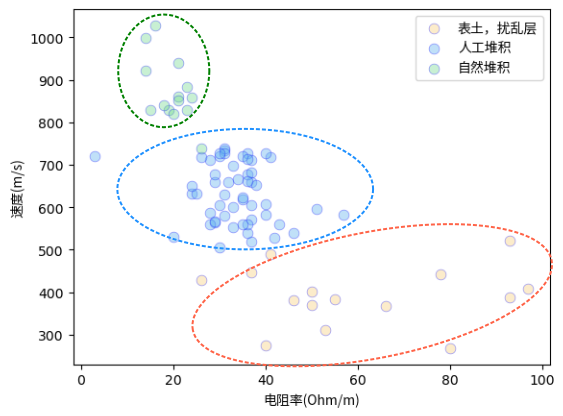
\includegraphics[width=0.8\textwidth]{figure/thesis/output_revised.png}
    \caption{良渚遗址--中心古城区钻孔物性交会图,中心古城区浅层可分为三大类:红色虚线—浅表杂土层、浅蓝色虚线—人工堆积层和绿色虚线—自然堆积层}
    \label{fig:pro_intersection}
\end{figure}

\subsection{FCM聚类联合反演}

在联合反演之前,我们需要确定目标函数的各项系数。如(\ref{fcmformula})所表示的,如果数据和先验信息完整,那么需要确定五组参数:地震数据和电法数据项的权重、震法和电法的正则化项权重和一组耦合系数。我以以下方法确定反演参数:

\begin{itemize}
    \item 利用单独反演的L曲线法确定每种反演方法的正则化项权重
    \item 进行无耦合的联合反演。如果目标函数收敛,我们就可以选择两者下降速度基本一致的两组权重系数以作为数据项的权重。
    \item 利用L曲线法,即在保证其他项获取的权重系数比例固定的情况下,计算耦合项和所有数据项的L曲线图。
\end{itemize}

通过上面的步骤,我们得到了联合反演目标函数的权重。我编不下去了。
